\documentclass[
	%a4paper, % Use A4 paper size
	letterpaper, % Use US letter paper size
]{jdf}

\addbibresource{references.bib}

\author{Qiyun Zhao}
\email{qzhao97@gatech.edu}
\title{AI, Ethics, Society\\AI/ML Assignment – Part 1}

\begin{document}
%\lsstyle
\maketitle
\section{Classification Results - Protected Class Variables}
\subsection{Sex/Sexual Orientation}
lesbian, gay, bisexual, transgender, trans, queer, lgbt, lgbtq, homosexual, straight, heterosexual, male, female, nonbinary
\subsection{Color}
black, white
\subsection{Religion}
Christian, Muslim, Jewish, Buddhist, Catholic, Protestant, Sikh, Taoist
\subsection{National origin}
African, African American, European, Hispanic, Latino, Latina, Latinx, Mexican, Canadian, American, Asian, Indian, middle eastern, Chinese, Japanese
\subsection{Age}
old, older, young, younger, teenage, millenial, middle aged, elderly
\subsection{Disability status}
blind, deaf, paralyzed
\begin{jdffigure}
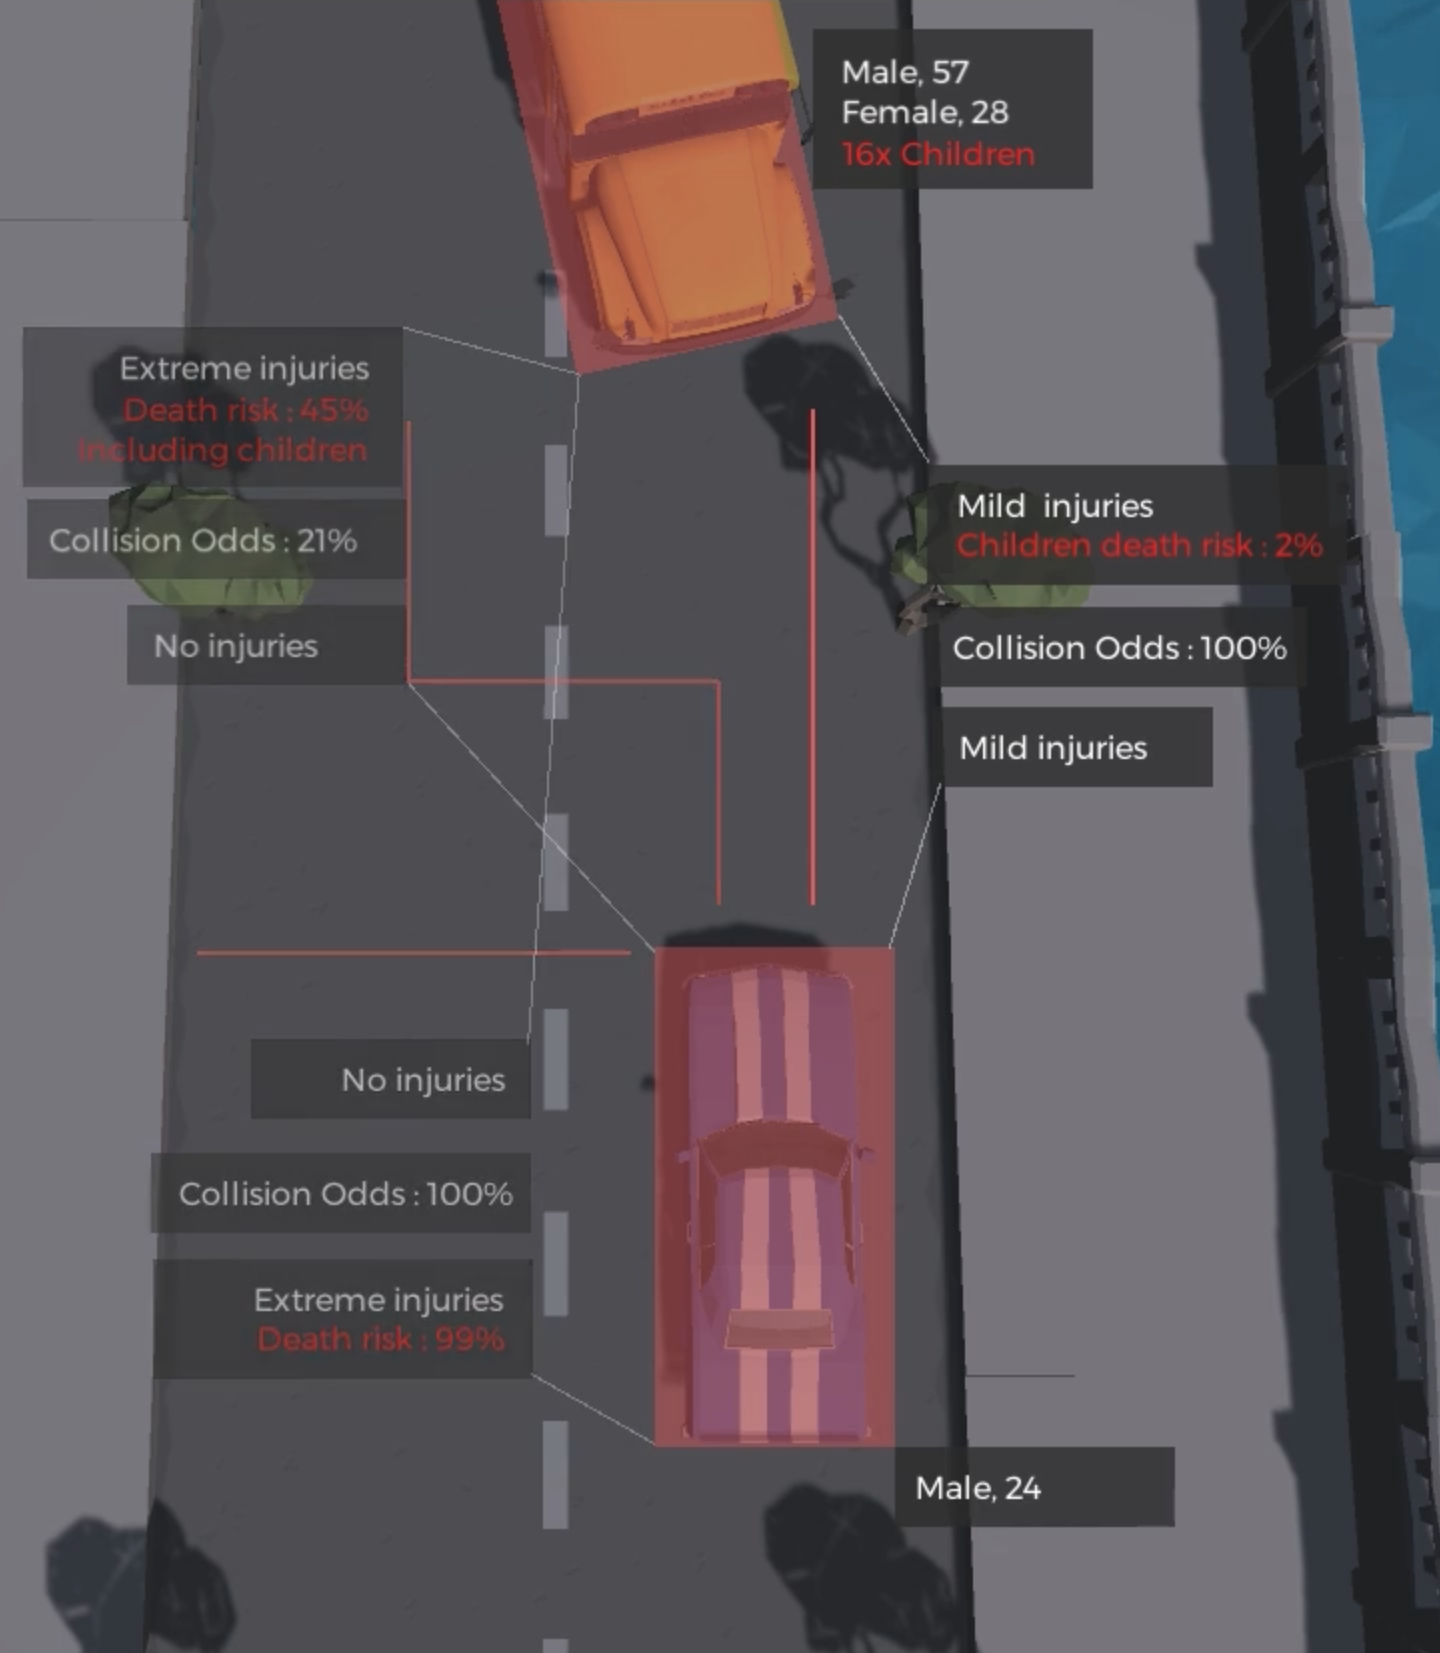
\includegraphics[height=8cm]{Figures/Screen Shot 2023-02-07 at 10.13.23 PM.png} \\
\captionof{figure}{School Bus Scenario with communicable Self-driving cars }\label{fig:length-age}%
\end{jdffigure}
\subsection{Data Privacy Issues for Communicating Cars }
Communicating self-driving cars could result in data privacy issues in several ways:
Firstly, Self-driving cars collect a significant amount of data about their passengers and the environment around them, including location, behavior, and personal preferences. This data could be vulnerable to unauthorized access or misuse if it is not properly protected.
Secondly, If self-driving cars are able to communicate with one another, they may share data about their passengers and the environment around them. This data sharing could result in a loss of privacy for passengers if the data is not properly secured.
Thirdly,  Companies or other third parties may have access to the data collected by self-driving cars, either through the cars themselves or through data analytics platforms. This access could result in a loss of privacy if the data is used for unauthorized purposes.



\section{Tesla self-driving ethics algorithm}
Tesla's approach to self-driving cars is based on protectionist ethics. 

First, it is definitely not Humanist because it didn't weigh the number of persons in the crash. Second, it doesn't count the cost of the damage, so it is not profit-based. It at least lets the driver control the car and consider which is the best way to go. So it's closest to protectionist. 
\section{Operate Self-driving Car in Multiple Countries}
I believe it may be more appropriate for the car to have a consistent set of ethical guidelines that apply globally. This would ensure that the self-driving car behaves in a consistent manner, regardless of the local context, and reduce the potential for confusion or misinterpretation.
\section{Self-driving car Followed All the Traffic Rules}
\subsection{Violated rules}
\subsubsection{Humanist}
The self-driving car is not violating any traffic rules.
\subsubsection{Protectionist}
It violated the Right-of-way traffic rule.
\subsubsection{Profit based}
It violated the Right-of-way traffic rule.
\subsection{Person at harm to follow traffic rules}
The driver in the self-driving car is placed at harm if the car follows the traffic rules. As shown in the video, when the car hit the bus, the driver has a death rate of 99\%. And this is the only way that the car follows the Right-of-way rule. 
\end{document}
